\section{Description of instrumental DetChar}

I did a whole lot of instrumental DetChar.

\section{Tools and algorithms}

\subsection{Omicron}

We use a sine-Gaussian basis to search for excess power

\subsection{Hveto}

Time correlations are used to search for auxiliary channels with glitches that 
correlate with DARM.

\section{Analog-to-Digital Conversion}

Advanced LIGO interferometers are controlled in real-time using a digital control system installed on a series of computers referred to as front end computers.  This system overall is referred to as the Front End Control (FEC) subsection of the more expansive Control and Data System (CDS).  In a control loop, the FE computers must be capable of reading in an analog signal from the interferometer (position measurements, error signals, coil currents, etc), digitally sampling that analog signal, using these now digital values in a series of control algorithms, and outputting an analog control signal to send back into the interferometer.

The process of digital sampling is handled by an analog-to-digital converter (ADC) and the process of analog output is handled by a digital-to-analog converter (DAC).  Since these converters are linearly mapping a continuous signal onto a discrete range, they are limited by their digital bit depth.  For example, a 16 bit ADC is only capable of representing $2^{16}$ discrete values, or a range from zero to 65536.  This range is often centered around zero, giving the ADC the capability to handle a range of $\pm32768$.  An incoming analog signal is mapped onto this range and converted into a digital signal.

For example, if I was sampling an analog signal with a range of $\pm100V$, 100V would be mapped to 32768 and -100V would be mapped to -32768 with all of the intermediate voltage values being linearly mapped to the range. This means our digital system would recognize a discrete step size of $100/32768 \approx 3.05 mV$.

Looking at the system described above, we must be aware of how our system is going to react when our analog input signal exceeds the intended maximum value of 100V (e.g., a 110V input). The ADC has already assigned its maximum digital value to 100V. This is called range saturation. In this case the ADC will continuously output its maximum value as it has no way to map 110V into a discrete value. The same process can occur in a DAC when a digital signal is sent out at the maximum allowed digital value.

If the digital system is not able to correctly sample and understand an analog error signal, it is easy to imagine a scenario where the reponse of the digital system and the output control signal are not able to complete the control loop as designed. This may cause glitches or misalignments.

We must also consider the fact that many ADCs are calibrated to reflect the intended dynamic range of an optic.  If a saturation is occurring, there is a good chance that an optic has moved beyond this intended dynamic range, which also may cause glitches or misalignments.

The ADCs and DACs are monitored by a series of auxiliary channels.  The most useful channels are of the form:

\begin{verbatim}
L1:FEC-21_DAC_OVERFLOW_0_0
\end{verbatim}

Parsing this channel name:

\begin{verbatim}
L1:FEC-{model number}_{ADC/DAC}_OVERFLOW_{ADC/DAC number}_{channel number}
\end{verbatim}

These overflow monitor channels are cumulative. If the channel has no saturation at the time of sampling, the overflow channel's reported value will not increase. If the channel was saturated during the last sample, the value of the channel will increase in discrete steps equal in size to the maximum value of the channel.


\textcolor{red}{Discuss Hveto results}

Used this to generate flags for veto definer, ETMY driver and OMC DCPD saturations.

\section{Suspension DAC calibration glitches}

We see glitches when suspensions cross values of zero or $2^{16}$.

\textcolor{red}{Discuss Hveto results}

\section{RF beatnote whistles}

Two RF oscillators beating against one another creates a kHz beatnote that couples 
into DARM.

\begin{figure}[ht!]%
\centering
\subfloat[]{
  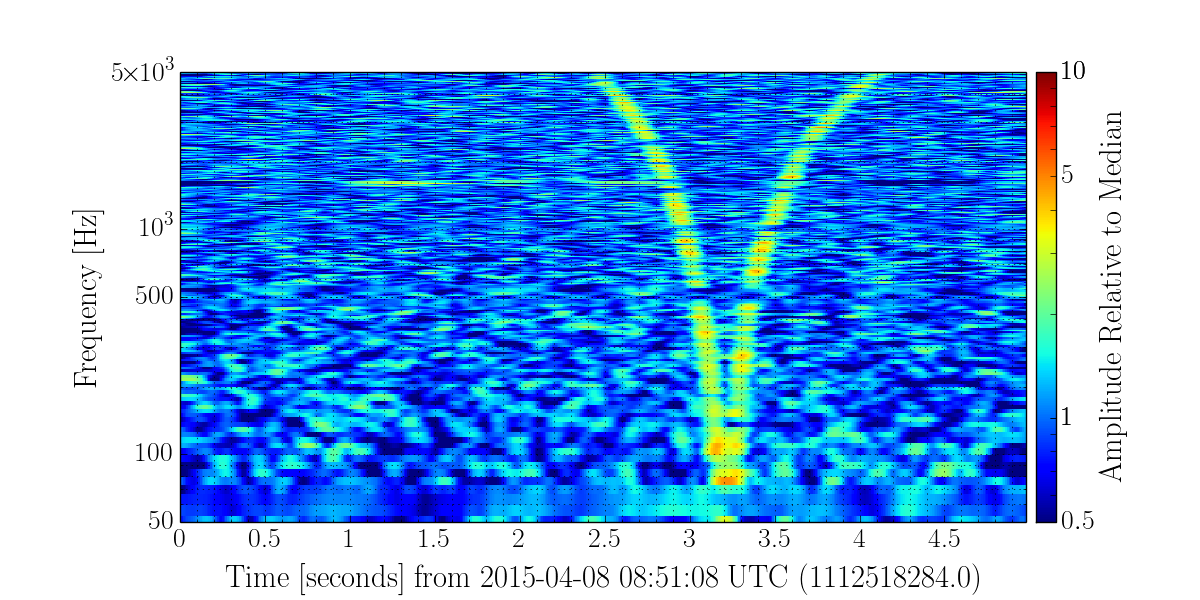
\includegraphics[width=\textwidth]{figures/detchar/Spectrogram_Whistle_LLO}
  \label{subfig:llo-whistle}
  }
  
\subfloat[]{
  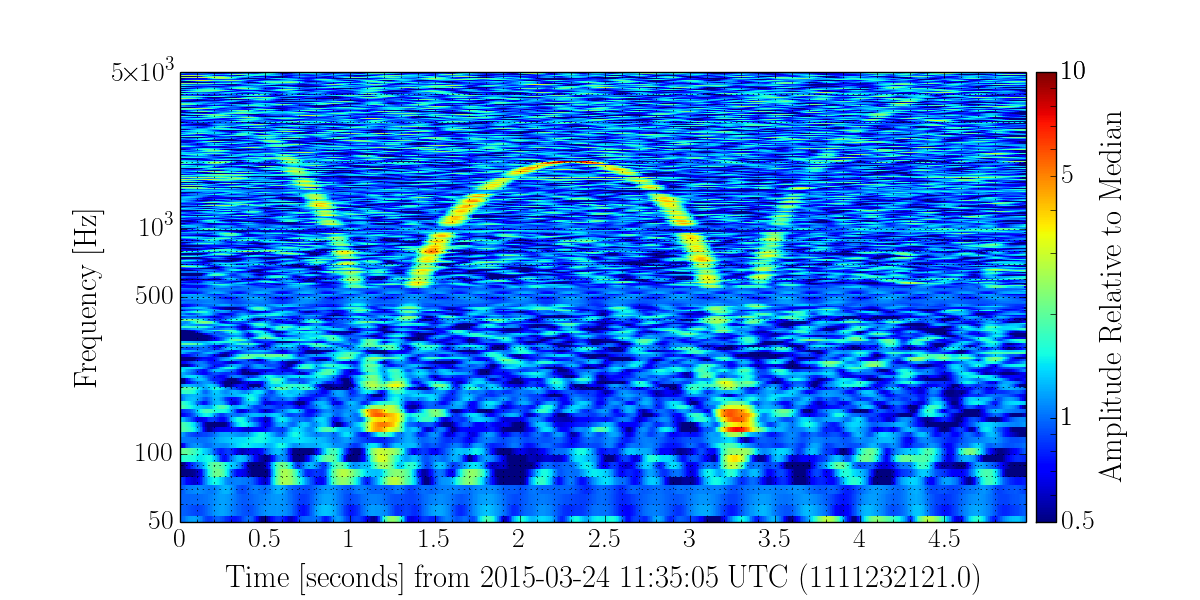
\includegraphics[width=\textwidth]{figures/detchar/Spectrogram_Whistle_LHO}
  \label{subfig:lho-whistle}
  }
\caption[Spectrograms of RF whistles]{Spectrograms of RF whistles at %
         both LLO and LHO. Figure \ref{subfig:llo-whistle} shows a %
         whistle at LLO. Figure \ref{subfig:lho-whistle} shows a whistle %
         at LHO.
         }
\end{figure}\label{fig:whistle-spectrograms}

\section{Seismic CPS comb}

Oscillators in the capacitive position sensors had drifted apart and caused a 
beatnote and a comb. Audio analysis pointed towards amplitude modulation. 

Fixed by slaving all oscillators to a master.

\section{DC values of auxiliary channels}

No great correlation at the end of the day 

\section{Earthquakes during full lock}

Lots of scattering arches during an earthquake, drove up the noise and biased PSD.
Caused a sarlacc, removing this data was able to repair data on either side.

\section{L1 PMC glitches}


Characterization of noise and analysis after repair

\section{Data quality shifts}
Performed and mentored data quality shifts.



